\documentclass[12pt, a4paper]{article}\usepackage[]{graphicx}\usepackage[]{color}
%% maxwidth is the original width if it is less than linewidth
%% otherwise use linewidth (to make sure the graphics do not exceed the margin)
\makeatletter
\def\maxwidth{ %
  \ifdim\Gin@nat@width>\linewidth
    \linewidth
  \else
    \Gin@nat@width
  \fi
}
\makeatother

\definecolor{fgcolor}{rgb}{0.345, 0.345, 0.345}
\newcommand{\hlnum}[1]{\textcolor[rgb]{0.686,0.059,0.569}{#1}}%
\newcommand{\hlstr}[1]{\textcolor[rgb]{0.192,0.494,0.8}{#1}}%
\newcommand{\hlcom}[1]{\textcolor[rgb]{0.678,0.584,0.686}{\textit{#1}}}%
\newcommand{\hlopt}[1]{\textcolor[rgb]{0,0,0}{#1}}%
\newcommand{\hlstd}[1]{\textcolor[rgb]{0.345,0.345,0.345}{#1}}%
\newcommand{\hlkwa}[1]{\textcolor[rgb]{0.161,0.373,0.58}{\textbf{#1}}}%
\newcommand{\hlkwb}[1]{\textcolor[rgb]{0.69,0.353,0.396}{#1}}%
\newcommand{\hlkwc}[1]{\textcolor[rgb]{0.333,0.667,0.333}{#1}}%
\newcommand{\hlkwd}[1]{\textcolor[rgb]{0.737,0.353,0.396}{\textbf{#1}}}%
\let\hlipl\hlkwb

\usepackage{framed}
\makeatletter
\newenvironment{kframe}{%
 \def\at@end@of@kframe{}%
 \ifinner\ifhmode%
  \def\at@end@of@kframe{\end{minipage}}%
  \begin{minipage}{\columnwidth}%
 \fi\fi%
 \def\FrameCommand##1{\hskip\@totalleftmargin \hskip-\fboxsep
 \colorbox{shadecolor}{##1}\hskip-\fboxsep
     % There is no \\@totalrightmargin, so:
     \hskip-\linewidth \hskip-\@totalleftmargin \hskip\columnwidth}%
 \MakeFramed {\advance\hsize-\width
   \@totalleftmargin\z@ \linewidth\hsize
   \@setminipage}}%
 {\par\unskip\endMakeFramed%
 \at@end@of@kframe}
\makeatother

\definecolor{shadecolor}{rgb}{.97, .97, .97}
\definecolor{messagecolor}{rgb}{0, 0, 0}
\definecolor{warningcolor}{rgb}{1, 0, 1}
\definecolor{errorcolor}{rgb}{1, 0, 0}
\newenvironment{knitrout}{}{} % an empty environment to be redefined in TeX

\usepackage{alltt}

%%%%%%%%%%%%%%%%%%%%%%%%%%%%%%%%%%%%%%%%%%%%%%%%%%%%%%%%%%%%%%%%
% LaTeX packages
%\usepackage[OT4]{polski}
\usepackage[utf8]{inputenc}
\usepackage[top=2.5cm, bottom=2.5cm, left=2cm, right=2cm]{geometry}
\usepackage{graphicx}
\usepackage{amsmath}
\usepackage{float}
\usepackage[colorlinks=true, linkcolor=blue]{hyperref}


%%%%%%%%%%%%%%%%%%%%%%%%%%%%%%%%%%%%%%%%%%%%%%%%%%%%%%%%%%%%%%%%
% global settings


\newtheorem{lemma}{Lemma}
\IfFileExists{upquote.sty}{\usepackage{upquote}}{}
\begin{document}

%%%%%%%%%%%%%%%%%%%%%%%%%%%%%%%%%%%%%%%%%%%%%%%%%%%%%%%%%%%%%%%%
% title page
\title{Estimation theory -- Report 4}
\author{Marta Frankowska, 208581 \\ Agnieszka Szkutek, 208619}
\maketitle
\tableofcontents 


%%%%%%%%%%%%%%%%%%%%%%%%%%%%%%%%%%%%%%%%%%%%%%%%%%%%%%%%%%%%%%%%

\section{Exercise 1}
We generate a time series of 20 observations according to the model $y_t = \alpha + \varepsilon_t$, where $\varepsilon_t \sim N(0,\sigma^2)$ and $iid$.

\subsection{Part 1}
The density function of a single observation is 
\[ f(y_t,\theta) = \frac{1}{\sqrt{2\pi\sigma^2}} e^{-\frac{(y_t-\alpha)^2}{2\sigma^2}},  \]
the likelihood function is 
\begin{gather*} 
L(\theta; y_1,\dots,y_N) = f(y_1,\dots,y_N; \theta) = \prod_{i=1}^{N} f(y_i; \theta) = \\
= \frac{1}{\sqrt{2\pi\sigma^2}} e^{-\frac{(y_1-\alpha)^2}{2\sigma^2}} \dots  \frac{1}{\sqrt{2\pi\sigma^2}} e^{-\frac{(y_N-\alpha)^2}{2\sigma^2}}
=  \left(\frac{1}{\sqrt{2\pi\sigma^2}} \right)^N e^{-\frac{1}{2\sigma^2} \sum_{i=1}^N (y_i-\alpha)^2} ,
\end{gather*}
and the log-likelihood is as follows
\[ l(\theta; y_1,\dots,y_N) = \ln{L(\theta; y_1,\dots,y_N)} = -\frac{N}{2} \ln{2\pi} -\frac{N}{2} \ln{\sigma^2} -\frac{1}{2\sigma^2} \sum_{i=1}^N (y_i-\alpha)^2.\]


\subsection{Part 2}
The contour plot of log-likelihood function is displayed below.
\begin{knitrout}
\definecolor{shadecolor}{rgb}{0.969, 0.969, 0.969}\color{fgcolor}\begin{figure}[H]

{\centering 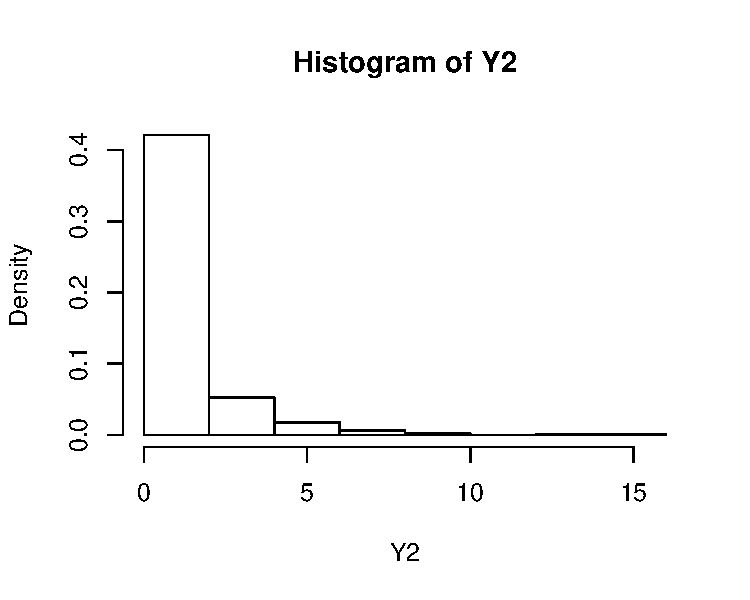
\includegraphics[width=\maxwidth]{figure/ex1_2-1} 

}

\caption[Contour plot of log-likelihood function]{Contour plot of log-likelihood function. The red point marks the maksimum of the function.}\label{fig:ex1.2}
\end{figure}


\end{knitrout}


\subsection{Part 3}
The First Order Condition is as follows $\frac{\partial \ln L}{\partial \theta} $, where vector $\theta$ is equal to
$ \theta = 
  \begin{bmatrix}  
    \alpha\\
    \sigma^2
  \end{bmatrix} $.
% 
%
It gives the following set of equations
\begin{gather*}
\begin{cases}
  \frac{\partial \ln L}{\partial \alpha} = 0 \\
  \frac{\partial \ln L}{\partial \sigma^2} = 0 
  \end{cases}
\ \Rightarrow \ 
\begin{cases}
  \frac{1}{\sigma^2} \sum_{i=1}^N (y_i-\alpha) = 0 \\
  -\frac{N}{2\sigma^2} + \frac{1}{2(\sigma^2)^2} \sum_{i=1}^N (y_i-\alpha)^2 = 0
\end{cases}
\ \Rightarrow \ 
\begin{cases}
  \frac{N}{N} \sum_{i=1}^N y_i - N \alpha = 0\\
  \frac{1}{\sigma^2} \sum_{i=1}^N (y_i-\alpha)^2 = N
\end{cases} \\
\ \Rightarrow \ 
\begin{cases}
  N (\bar{y}-\alpha) = 0\\
  \sigma^2 = \frac{1}{N} \sum_{i=1}^N (y_i-\alpha)^2
\end{cases}
\ \Rightarrow \ 
\begin{cases}
  \alpha = \bar{y} \\
  \sigma^2 = \frac{1}{N} \sum_{i=1}^N (y_i-\bar{y})^2
\end{cases}
\end{gather*}
%
So the ML estimators of the model parameters are
\[ \begin{cases}
  \hat{\alpha} = \bar{y}\\
  \hat{\sigma}^2 = \frac{1}{N} \sum_{i=1}^N (y_i-\bar{y})^2
\end{cases}
\]




\subsection{Part 4}
\subsubsection{Variance-covariance matrix}

The variance-covariance matrix of parameters $\hat{\alpha}$ and $\hat{\sigma}^{2}$:
\[
  \Sigma_{(\hat{\alpha},\hat{\sigma}^{2})}=
  \begin{bmatrix}  
    Var\hat{\alpha} & Cov(\hat{\alpha},\hat{\sigma}^{2})\\
    Cov(\hat{\alpha},\hat{\sigma}^{2}) & Var\hat{\sigma}^{2}
  \end{bmatrix},
\]
where $ Var\hat{\alpha}=Var\bar{y}=Var\left(\frac{1}{N}\sum^{N}_{i=1}y_{i}\right)=\frac{\sigma^{2}}{N} $.

We know that $\frac{N\hat{\sigma}^{2}}{\sigma^{2}}\sim\chi^{2}(N-1)$ and $Var[\chi^{2}(N-1)]=2(N-1)$ so
\[
Var\left(\frac{N\hat{\sigma}^{2}}{\sigma^{2}}\right)=\frac{N^2}{\sigma^{4}}Var(\hat{\sigma}^{2})=2(N-1)
\quad \Rightarrow \quad
Var(\hat{\sigma}^{2})=\frac{2(N-1)\sigma^{4}}{N^{2}}
\]
To calculate $Cov(\hat{\alpha},\hat{\sigma}^{2})$ we will use the following fact.
%
\begin{lemma}
Let $X_{1},...,X_{N}\sim N(\mu,\sigma^{2})$.
Then $\bar{X}=\frac{1}{N}\sum_{i=1}^{N}X_{i}$ and $\hat{\sigma}^{2}=\frac{1}{N}\sum_{i=1}^{N}(X_i-\bar{X})^{2}$ are independent. 
That means $Cov(\bar{X},\hat{\sigma}^{2})=0$.
\end{lemma}
%
Thus the variance-covariance matrix of parameters $\hat{\alpha}$ and $\hat{\sigma}^{2}$ is
\[
  \Sigma_{(\hat{\alpha},\hat{\sigma}^{2})}=
  \begin{bmatrix}  
    \sigma^{2} & 0\\
    0 & \frac{2(N-1)\sigma^{4}}{N^{4}}
  \end{bmatrix}.
\]
Substituting $\sigma^2 = Var(Y)$ and $N$ equal to length of the data we obtain the sample variance-covariance matix 
\begin{knitrout}
\definecolor{shadecolor}{rgb}{0.969, 0.969, 0.969}\color{fgcolor}\begin{kframe}
\begin{verbatim}
##          [,1]        [,2]
## [1,] 2.991618 0.000000000
## [2,] 0.000000 0.002125572
\end{verbatim}
\end{kframe}
\end{knitrout}



\subsubsection{The asymptotic distribution of ML estimator}

The asymptotic distribution of ML estimator is
\[\hat{\theta}\xrightarrow[]{d}N(\theta_0, I(\theta_0)^{-1}),\]
where $I(\theta_{0}) = -E_0(H(\theta_{0})) = -E_0\left(\frac{\partial^{2}\ln{L}}{\partial\theta_{0}\partial\theta_{0}'}\right)$.

We calculate partial derivatives:
\begin{align*}
\frac{\partial\ln{L}}{\partial\alpha}=\frac{1}{\sigma^2}N(\bar{y}-\alpha), & \quad \frac{\partial^{2}\ln{L}}{\partial\alpha^{2}}=-\frac{N}{\sigma^{2}} \\
\frac{\partial\ln{L}}{\partial\sigma^{2}}=-\frac{N}{2\sigma^{2}}+\frac{1}{2\sigma^{4}}\sum_{i=1}^{N}(y_{i}-\alpha)^{2}, & \quad
  \frac{\partial^{2}\ln{L}}{\partial(\sigma^{2})^{2}}=\frac{N}{2\sigma^{4}}-\frac{1}{(\sigma^{2})^{3}}\sum_{i=1}^{N}(y_{i}-\alpha)^2 \\
\frac{\partial^{2}\ln{L}}{\partial\alpha\partial\sigma^{2}} =\frac{\partial^{2}\ln{L}}{\partial\sigma^{2}\partial\alpha}=&-\frac{1}{\sigma^{4}}\sum_{i=1}^{N}(y_{i}-\alpha)
\end{align*}

Now we calculate expected value of the above derivatives:
\begin{align*}
E\frac{\partial^{2}\ln{L}}{\partial\alpha^{2}}=&-\frac{N}{\sigma^{2}} \\
%
E\frac{\partial^{2}\ln{L}}{\partial(\sigma^{2})^{2}}=&E\left(\frac{N}{2\sigma^{4}}\right)-E\left(\frac{1}{\sigma^{6}}\sum_{i=1}^{N}(y_{i}-\alpha)^{2}\right)=\frac{N}{2\sigma^{4}}-\frac{N}{\sigma^{4}}=-\frac{N}{2\sigma^{4}}\\
%
E\frac{\partial^{2}\ln{L}}{\partial\alpha\partial\sigma^{2}}=&-\frac{1}{\sigma^{4}}E\sum_{i=1}^{N}(y_{i}-\alpha)=-\frac{1}{\sigma^{4}}\sum_{i=1}^{N}E(y_{i}-\alpha)=0
\end{align*}
So 
\[
I^{-1}(\theta_{0})=
\begin{bmatrix}  
    \frac{N}{\sigma^{2}} & 0\\
    0 & \frac{N}{2\sigma^{4}}
  \end{bmatrix}^{-1}=
	\begin{bmatrix}  
    \frac{\sigma^{2}}{N} & 0\\
    0 & \frac{2\sigma^{4}}{N}
  \end{bmatrix}
\]
We see that asymptotic covariance of $\hat{\alpha}$ and $\hat{\sigma}^{2}$ is equal to 0.




\subsection{Part 5}

To calculate ML estimator of $1+\alpha+\alpha^{2}$ we use below property.
%
\begin{lemma}[Invariance property]
$\hat{g}(\theta)=g(\hat{\theta})$, where $\hat{\theta}$ is MLE of $\theta$ and $g$ is continous and continously differentaible funcion.
\end{lemma}
%
ML estimator of $\beta=1+\alpha+\alpha^{2}$ is 
\[\hat{\beta}=\hat{g}(\alpha)=g(\hat{\alpha})=1+\hat{\alpha}+\hat{\alpha}^{2}=1+\bar{y}+\bar{y}^{2}.\]
%
Now we calculate $Var\hat{\beta}$ using fact that $\hat{\alpha}\sim N(\alpha,\frac{\sigma^{2}}{N})$.
%
\begin{gather*}
Var(\hat{\beta})=Var(1+\hat{\alpha}+\hat{\alpha}^{2})=Var(\hat{\alpha}+\hat{\alpha}^{2})=E(\hat{\alpha}+\hat{\alpha}^{2})^{2}-(E(\hat{\alpha}+\hat{\alpha}^{2}))^{2}=\\
=E\hat{\alpha}^{2}+2E\hat{\alpha}^{3}+E\hat{\alpha}^{4}-(E\hat{\alpha})^{2}-2E\hat{\alpha}E\hat{\alpha}^{2}-(E\hat{\alpha}^{2})^{2}
\end{gather*}
Using formula for normal distribution moments we get
\[ E\hat{\alpha}=\alpha ,\quad E\hat{\alpha}^{2}=\alpha^{2}+\frac{\sigma^{2}}{N} ,\quad E\hat{\alpha}^{3}=\alpha^{3}+3\alpha\frac{\sigma^{2}}{N} ,\quad\text{and}\quad
E\hat{\alpha}^{4}=\alpha^{4}+6\alpha^{2}\frac{\sigma^{2}}{N}+3\frac{\sigma^{4}}{N^{2}},
\]
and
\begin{gather*}
Var(\hat{\beta})=\alpha^{2}+\frac{\sigma^{2}}{N}+2\alpha^{3}+6\alpha\frac{\sigma^{2}}{N}+\alpha^{4}+6\alpha^{2}\frac{\sigma^{2}}{N}+3\frac{\sigma^{4}}{N^{2}}
-\alpha^{2}-2\alpha\left(\alpha^{2}-\frac{\sigma^{2}}{N}\right) -\left(\alpha^{2}+\frac{\sigma^{2}}{N}\right)^{2}= \\
= \frac{\sigma^{2}}{N}+4\alpha\frac{\sigma^{2}}{N}+4\alpha^{2}\frac{\sigma^{2}}{N}+2\frac{\sigma^4}{N^{2}}.
\end{gather*}


%%%%%%%%%%%%%%%%%%%%%%%%%%%%%%%%%%%%%%%%%%%%%%%%%%%%%%%%%%%%%%%%%%%%%%%%%%%%%%%%%%%%%%%%%%%%%%%%%%%%%%%%%%%%%%%%%%%%%%%%%%%%%%%%
%%%%%%%%%%%%%%%%%%%%%%%%%%%%%%%%%%%%%%%%%%%%%%%%%%%%%%%%%%%%%%%%%%%%%%%%%%%%%%%%%%%%%%%%%%%%%%%%%%%%%%%%%%%%%%%%%%%%%%%%%%%%%%%%

\section{Exercise 2}
In this exercise we will be using data set from file \textit{datalab4-1.xlsx}. We will assume that $y$ has a mixed normal distribution,
\[ y_n \sim 
  \begin{cases}
    N(0,1), \quad\text{for } p \\
    N(\mu, \sigma^2), \quad\text{for } 1-p, \\
  \end{cases}
  \quad\text{depending on }
  \theta = \begin{bmatrix} \mu \\ \sigma^2 \\ p \end{bmatrix}.
\]

\subsection{Part 1}
The density function of $y$ is equal to
\[ f(y; \theta) = f(y; \mu, \sigma^2, p) = p\cdot  f(y; 0, 1) + (1-p) \cdot  f(y; \mu, \sigma^2), \]
where 
\[ f(y; \mu, \sigma^2) = \frac{1}{\sqrt{2\pi\sigma^2}} e^{-\frac{(y-\mu)^2}{2\sigma^2}} \]
is the density function for normal distribution with parameters $\mu$ and $\sigma^2$.


The likelihood function of $y$ is obtained in the following way
\begin{gather*} 
  L(\theta; y_1,\dots,y_N) = \prod_{i=1}^N f(y_i; \theta) = \prod_{i=1}^N  \left(  p\cdot  f(y_i; 0, 1) + (1-p) \cdot  f(y_i; \mu, \sigma^2) \right) = \\
  = \prod_{i=1}^N \left(  p\cdot  \frac{1}{\sqrt{2\pi}} e^{-\frac{y_i^2}{2}} + (1-p)\frac{1}{\sqrt{2\pi\sigma^2}} e^{-\frac{(y_i-\mu)^2}{2\sigma^2}}  \right).
\end{gather*}

The log-likelihood function of $y$ is as follows
\begin{gather*} 
  l(\theta; y_1,\dots,y_N) = \log{L(\theta; y_1,\dots,y_N)} = \log \prod_{i=1}^N f(y_i; \theta) = \sum_{i=1}^N \log f(y_i; \theta) = \\
  \sum_{i=1}^N \log \left(  p\cdot  f(y_i; 0, 1) + (1-p) \cdot  f(y_i; \mu, \sigma^2) \right).
\end{gather*}

\subsection{Part 2}
In the left plot we took $\sigma = [0.01,0.02,0.03,\dots,4]$ and in the right $\sigma = [e^{-1}, e^{-2}, e^{-3},\dots, e^{-N}]$, where $N$ is the length of the data.
\begin{knitrout}
\definecolor{shadecolor}{rgb}{0.969, 0.969, 0.969}\color{fgcolor}\begin{figure}[H]

{\centering \includegraphics[width=\maxwidth]{figure/ex2_2-1} 

}

\caption[Log-likelihood function for different values of sigma]{Log-likelihood function for different values of sigma}\label{fig:ex2.2}
\end{figure}


\end{knitrout}

\begin{gather*}
L(\theta; y_1,\dots,y_N)
  = \prod_{i=1}^N \left(  p  \frac{1}{\sqrt{2\pi}} e^{-\frac{y_i^2}{2}} + (1-p)\frac{1}{\sqrt{2\pi\sigma^2}} e^{-\frac{(y_i-\mu)^2}{2\sigma^2}}  \right) = \\
  = \left(  p  \frac{1}{\sqrt{2\pi}} e^{-\frac{y_1^2}{2}} + (1-p)\frac{1}{\sqrt{2\pi\sigma^2}} e^{-\frac{(y_1-\mu)^2}{2\sigma^2}}  \right) \cdots
    \left(  p  \frac{1}{\sqrt{2\pi}} e^{-\frac{y_N^2}{2}} + (1-p)\frac{1}{\sqrt{2\pi\sigma^2}} e^{-\frac{(y_N-\mu)^2}{2\sigma^2}}  \right)
\end{gather*}
We took $\mu = y_1$, so  
\[ \mu - y_1 = 0 \quad\Rightarrow\quad e^{-\frac{(y_1-\mu)^2}{2\sigma^2}} = e^0 = 1. \]
Then the second component of the sum is $(1-p)\frac{1}{\sqrt{2\pi\sigma^2}}$. But if we take $\sigma$ close to 0, then the whole fraction goes to infinity.
\begin{gather*} 
  (1-p)\frac{1}{\sqrt{2\pi\sigma^2}} \rightarrow^{\sigma\rightarrow 0}  \infty 
  \quad\Rightarrow\quad 
  \left(  p  \frac{1}{\sqrt{2\pi}} e^{-\frac{y_1^2}{2}} + (1-p)\frac{1}{\sqrt{2\pi\sigma^2}} e^{-\frac{(y_1-\mu)^2}{2\sigma^2}}  \right) \rightarrow^{\sigma\rightarrow 0} \infty \quad\Rightarrow\quad \\
  \quad\Rightarrow\quad 
  L(\theta; y_1,\dots,y_N) \rightarrow^{\sigma\rightarrow 0} \infty 
  \quad\Rightarrow\quad 
  \ln{L(\theta; y_1,\dots,y_N)} \rightarrow^{\sigma\rightarrow 0} \infty 
\end{gather*}
Then $l(\theta; y_1,\dots,y_N)$ goes to infinity, so maximum of $l(\theta; y_1,\dots,y_N)$ doesn't exist.


%%%%%%%%%%%%%%%%%%%%%%%%%%%%%%%%%%%%%%%%%%%%%%%%%%%%%%%%%%%%%%%%%%%%%%%%%%%%%%%%%%%%%%%%%%%%%%%%%%%%%%%%%%%%%%%%%%%%%%%%%%%%%%%%
%%%%%%%%%%%%%%%%%%%%%%%%%%%%%%%%%%%%%%%%%%%%%%%%%%%%%%%%%%%%%%%%%%%%%%%%%%%%%%%%%%%%%%%%%%%%%%%%%%%%%%%%%%%%%%%%%%%%%%%%%%%%%%%%

\section{Exercise 3}

We suppose that $y$ has a Bernoulli distribution
\[ y= 
\begin{cases}
  1, \quad F(x_n; \theta) \\
  0, \quad 1-F(x_n; \theta),
\end{cases}
\]
where $F(x_n; \theta) = \frac{e^{\theta_1 + x_n \theta_2}}{1+e^{\theta_1 + x_n \theta_2}}$ is the probability of success.

\subsection{Part 1}
The marginal effect of variable $x$ on the probability of success is given by the partial derivative
\begin{gather*} 
  \frac{\partial F(x; \theta)}{\partial x} =   
  \frac{\partial}{\partial x} \left(  \frac{e^{\theta_1 + x_n \theta_2}}{1+e^{\theta_1 + x_n \theta_2}}  \right) = 
  \frac{\theta_2 e^{\theta_1 + x_n \theta_2} (1+e^{\theta_1 + x_n \theta_2}) -  e^{\theta_1 + x_n \theta_2} \theta_2 e^{\theta_1 + x_n \theta_2} }
    {\left( 1+e^{\theta_1 + x_n \theta_2} \right)^2 } = \\ =
  \theta_2 e^{\theta_1 + x_n \theta_2} \frac{1+ e^{\theta_1 + x_n \theta_2} -e^{\theta_1 + x_n \theta_2} }
    {\left( 1+e^{\theta_1 + x_n \theta_2} \right)^2 } =
  \frac{\theta_2 e^{\theta_1 + x_n \theta_2}}{\left( 1+e^{\theta_1 + x_n \theta_2} \right)^2 }.
\end{gather*}


\subsection{Part 2}
The likelihood function is as follows
\[L(\theta;(x_{1},y_{1}),...,(x_{N},y_{N}))=\prod_{k=1}^{N}(F(x_{k};\theta))^{y_{k}}(1-F(x_{k};\theta))^{1-y_{k}}\]
so the log-likelihood function is 
\begin{gather*}
  l(\theta;(x_{1},y_{1}),...,(x_{N},y_{N}))=\sum_{k=1}^{N}(y_{k}\ln{F(x_{k};\theta)}+(1-y_{k})\ln{(1-F(x_{k};\theta))})=\\
    =\sum_{k=1}^{N}(y_{k}
      \ln{\frac{e^{\theta_{1}+x_{k}\theta_{2}}}{1+e^{\theta_{1}+x_{k}\theta_{2}}}}
      +(1-y_{k})\ln{(1-\frac{e^{\theta_{1}+x_{k}\theta_{2}}}{1+e^{\theta_{1}+x_{k}\theta_{2}}}}))=\\
    =\sum_{k=1}^{N}(y_{k}(\theta_{1}+x_{k}\theta_{2})-y_{k}\ln{(1+e^{\theta_{1}+x_{k}\theta_{2}})}+\ln{1}-\ln{(1+e^{\theta_{1}+x_{k}\theta_{2}})}-\\
      -y_{k}\ln{1}+y_{k}\ln{(1+e^{\theta_{1}+x_{k}\theta_{2}})})
    =\sum_{k=1}^{N}(y_{k}(\theta_{1}+x_{k}\theta_{2})-\ln{(1+e^{\theta_{1}+x_{k}\theta_{2}})})
\end{gather*}


\subsection{Part 3}
We can see that we are not able to solve this set of equations analitically.
\[\frac{\partial l}{\partial\theta_{1}}=\sum_{k=1}^{N}(y_{k}-\frac{e^{\theta_{1}+x_{k}\theta_{2}}}{1+e^{\theta_{1}+x_{k}\theta_{2}}})=0\]
\[\frac{\partial l}{\partial\theta_{2}}=\sum_{k=1}^{N}(y_{k}x_{k}-\frac{e^{\theta_{1}+x_{k}\theta_{2}}x_{k}}{1+e^{\theta_{1}+x_{k}\theta_{2}}})=0\]



\subsection{Part 4}
Because we can't calculate $\theta_1$ and $\theta_2$ analitically, we will calculate the maximum of the log-likelihood function numerically using Newton's method.

The $\hat{\theta}_1$ and $\hat{\theta}_2$ are equal to
\begin{knitrout}
\definecolor{shadecolor}{rgb}{0.969, 0.969, 0.969}\color{fgcolor}\begin{kframe}
\begin{verbatim}
## [1] -0.2913384  1.0768976
\end{verbatim}
\end{kframe}
\end{knitrout}
We tested various starting points for the Newton's method to find $\hat{\theta}_1$ and $\hat{\theta}_2$ and the results were almost always the same, the error was $O(10^{-4})$.


\subsection{Part 5}
Using Newton's method we obtained also the hesian matix of the log-likelihood function and to estimate the variance-covariance matrix we use the following formula
$ \Sigma_{\hat{\theta}} = (-H(\hat{\theta}))^{-1}$.

\begin{knitrout}
\definecolor{shadecolor}{rgb}{0.969, 0.969, 0.969}\color{fgcolor}\begin{kframe}
\begin{verbatim}
##              [,1]         [,2]
## [1,]  0.071714628 -0.007825794
## [2,] -0.007825794  0.046786323
\end{verbatim}
\end{kframe}
\end{knitrout}



\subsection{Part 6}
The estimated marginal effect of $x$ on $y$ using $\hat{\theta}_1$, $\hat{\theta}_2$ and $\bar{x}$ is equal to
\begin{knitrout}
\definecolor{shadecolor}{rgb}{0.969, 0.969, 0.969}\color{fgcolor}\begin{kframe}
\begin{verbatim}
## [1] 0.4643691
\end{verbatim}
\end{kframe}
\end{knitrout}





\end{document}
